\documentclass{standalone}
\usepackage{tikz}
\usetikzlibrary{patterns, positioning}
\usepackage[sfdefault]{ClearSans} %% option 'sfdefault' activates Clear Sans as the default text font
\usepackage[T1]{fontenc}

\begin{document}
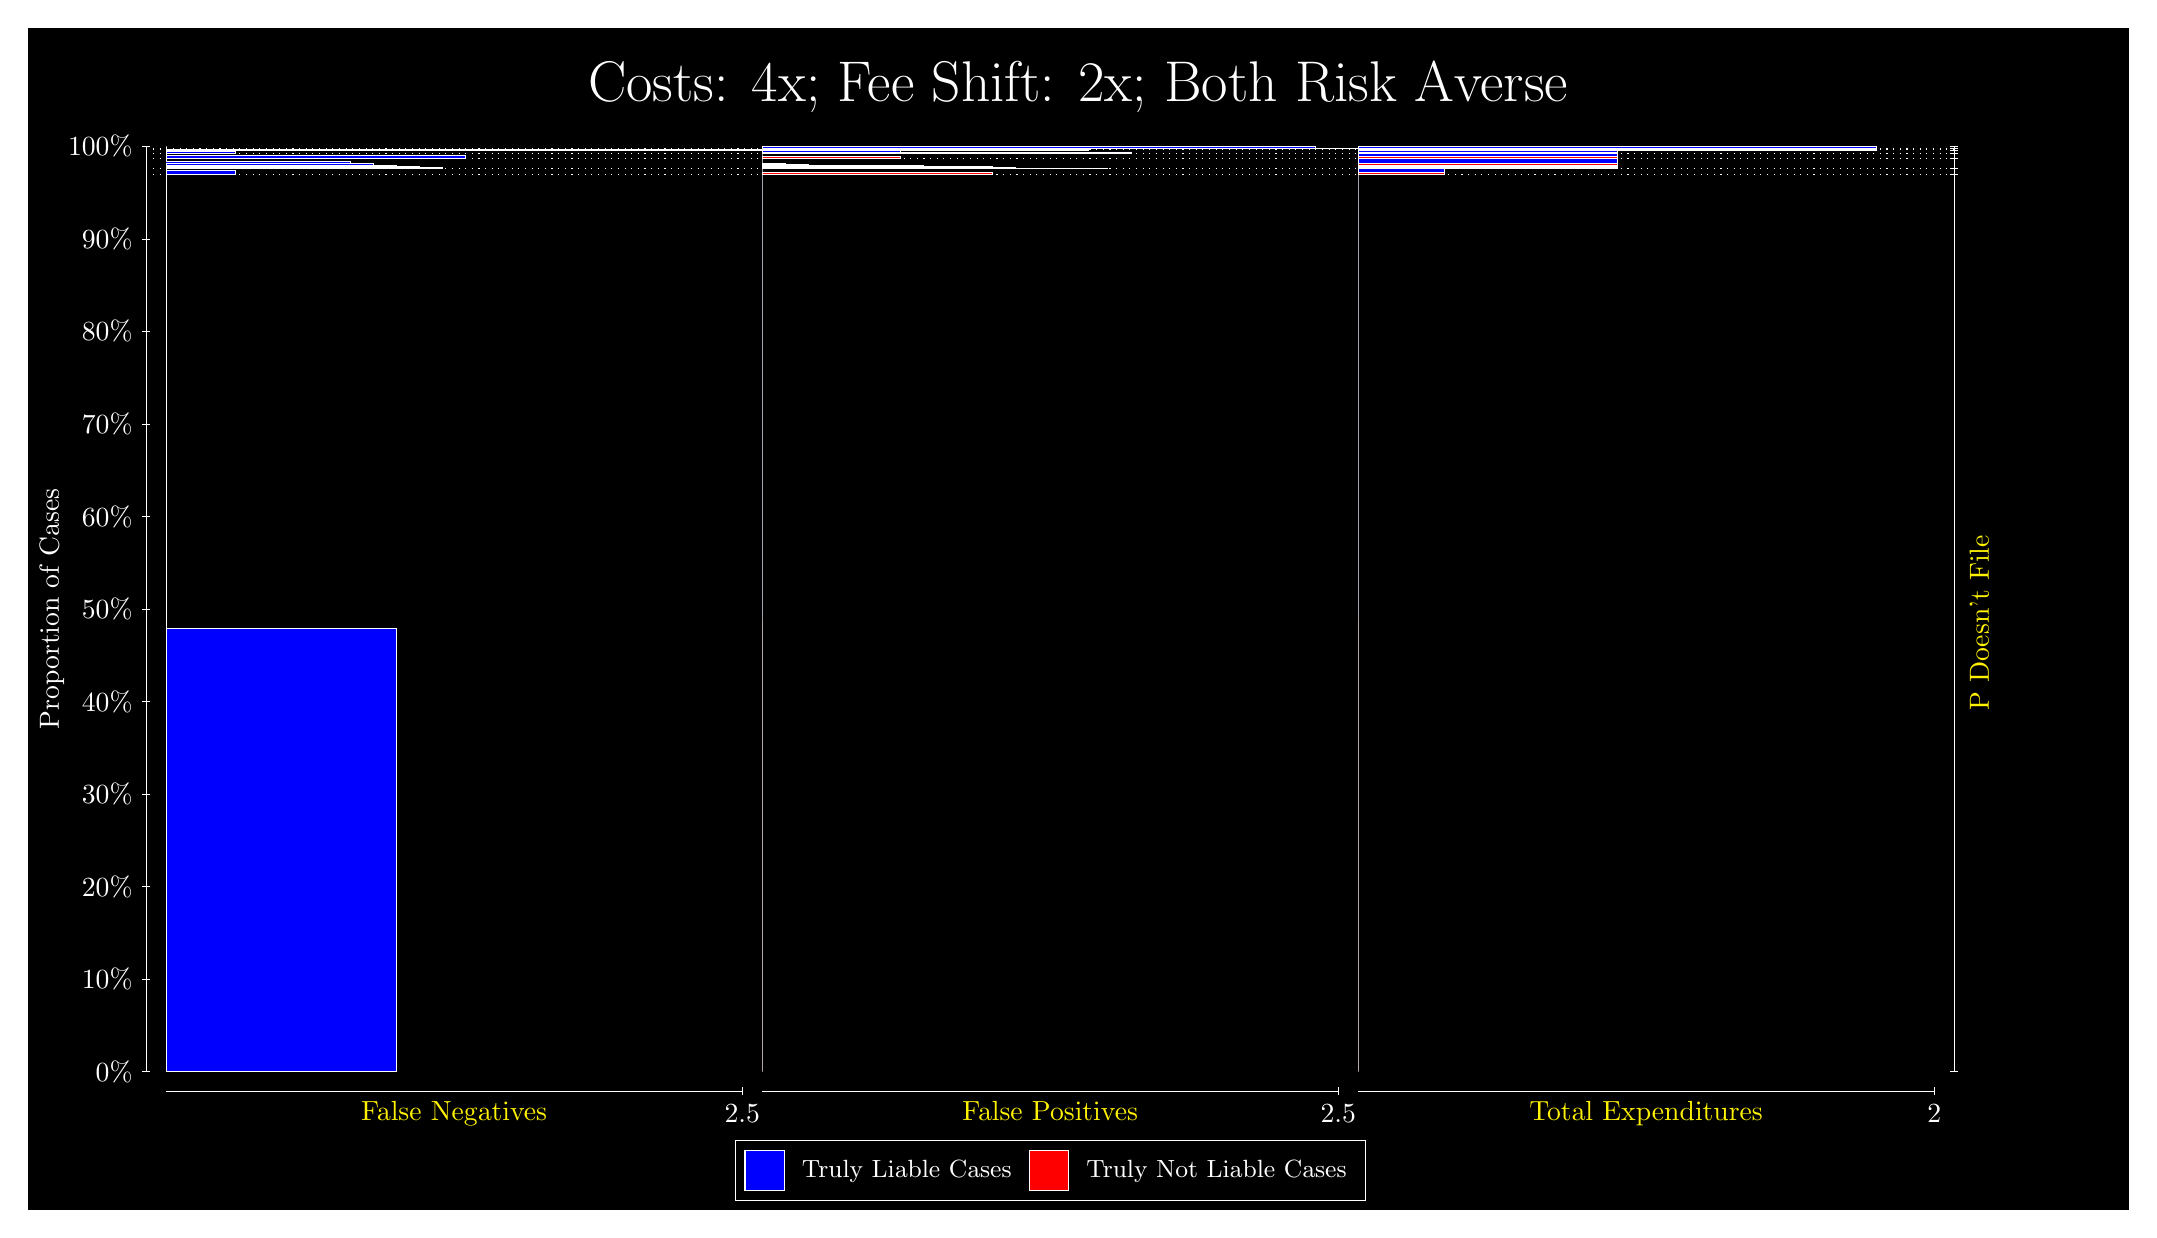
\begin{tikzpicture}
\draw[fill=black] (0,0) rectangle (26.667,15);
\draw[text=white] (0,13.5) rectangle (26.667,15) node[midway] {\huge Costs: 4x; Fee Shift: 2x; Both Risk Averse};
\draw[white, very thin] (1.5,1.75) -- (1.5,13.5);
\node[rotate=90, text=white, anchor=center] at (0.3, 7.625) {Proportion of Cases};
\draw[white, very thin] (1.45,1.75) -- (1.55,1.75);
\node[text=white, anchor=east] at (1.45, 1.75) {0\%};
\draw[white, very thin] (1.45,2.925) -- (1.55,2.925);
\node[text=white, anchor=east] at (1.45, 2.925) {10\%};
\draw[white, very thin] (1.45,4.1) -- (1.55,4.1);
\node[text=white, anchor=east] at (1.45, 4.1) {20\%};
\draw[white, very thin] (1.45,5.275) -- (1.55,5.275);
\node[text=white, anchor=east] at (1.45, 5.275) {30\%};
\draw[white, very thin] (1.45,6.45) -- (1.55,6.45);
\node[text=white, anchor=east] at (1.45, 6.45) {40\%};
\draw[white, very thin] (1.45,7.625) -- (1.55,7.625);
\node[text=white, anchor=east] at (1.45, 7.625) {50\%};
\draw[white, very thin] (1.45,8.8) -- (1.55,8.8);
\node[text=white, anchor=east] at (1.45, 8.8) {60\%};
\draw[white, very thin] (1.45,9.975) -- (1.55,9.975);
\node[text=white, anchor=east] at (1.45, 9.975) {70\%};
\draw[white, very thin] (1.45,11.15) -- (1.55,11.15);
\node[text=white, anchor=east] at (1.45, 11.15) {80\%};
\draw[white, very thin] (1.45,12.325) -- (1.55,12.325);
\node[text=white, anchor=east] at (1.45, 12.325) {90\%};
\draw[white, very thin] (1.45,13.5) -- (1.55,13.5);
\node[text=white, anchor=east] at (1.45, 13.5) {100\%};

\draw[white, very thin] (24.457,1.75) -- (24.457,13.5);
\draw[white, very thin] (24.407,1.75) -- (24.507,1.75);
\node[anchor=west] at (24.407, 1.75) {};
\draw[white, very thin] (24.407,13.143) -- (24.507,13.143);
\node[anchor=west] at (24.407, 13.143) {};
\draw[white, very thin] (24.407,13.223) -- (24.507,13.223);
\node[anchor=west] at (24.407, 13.223) {};
\draw[white, very thin] (24.407,13.348) -- (24.507,13.348);
\node[anchor=west] at (24.407, 13.348) {};
\draw[white, very thin] (24.407,13.411) -- (24.507,13.411);
\node[anchor=west] at (24.407, 13.411) {};
\draw[white, very thin] (24.407,13.455) -- (24.507,13.455);
\node[anchor=west] at (24.407, 13.455) {};
\draw[white, very thin] (24.407,13.47) -- (24.507,13.47);
\node[anchor=west] at (24.407, 13.47) {};
\draw[white, very thin] (24.407,13.5) -- (24.507,13.5);
\node[anchor=west] at (24.407, 13.5) {};

\draw[white, very thin, fill=blue] (1.75,1.75) rectangle (4.6775,7.3752);
\draw[white, very thin, fill=red] (1.75,7.3752) rectangle (1.75,13.143);
\draw[white, very thin, fill=blue] (1.75,13.143) rectangle (2.6283,13.199);
\draw[white, very thin, fill=red] (1.75,13.199) rectangle (1.75,13.223);
\draw[white, very thin, fill=blue] (1.75,13.223) rectangle (5.2631,13.236);
\draw[white, very thin, fill=blue] (1.75,13.236) rectangle (4.9703,13.241);
\draw[white, very thin, fill=blue] (1.75,13.241) rectangle (4.6775,13.263);
\draw[white, very thin, fill=blue] (1.75,13.263) rectangle (4.3848,13.265);
\draw[white, very thin, fill=blue] (1.75,13.265) rectangle (4.3848,13.283);
\draw[white, very thin, fill=blue] (1.75,13.283) rectangle (4.092,13.304);
\draw[white, very thin, fill=blue] (1.75,13.304) rectangle (3.7993,13.307);
\draw[white, very thin, fill=blue] (1.75,13.307) rectangle (3.5065,13.31);
\draw[white, very thin, fill=blue] (1.75,13.31) rectangle (3.2138,13.311);
\draw[white, very thin, fill=blue] (1.75,13.311) rectangle (2.921,13.313);
\draw[white, very thin, fill=red] (1.75,13.313) rectangle (1.75,13.348);
\draw[white, very thin, fill=blue] (1.75,13.348) rectangle (5.5558,13.391);
\draw[white, very thin, fill=red] (1.75,13.391) rectangle (1.75,13.411);
\draw[white, very thin, fill=blue] (1.75,13.411) rectangle (2.6283,13.443);
\draw[white, very thin, fill=red] (1.75,13.443) rectangle (1.75,13.455);
\draw[white, very thin, fill=blue] (1.75,13.455) rectangle (13.46,13.46);
\draw[white, very thin, fill=red] (1.75,13.46) rectangle (1.75,13.47);
\draw[white, very thin, fill=red] (1.75,13.47) rectangle (1.75,13.475);
\draw[white, very thin, fill=blue] (1.75,13.475) rectangle (1.75,13.5);
\draw[white, very thin, fill=red] (9.3189,1.75) rectangle (9.3189,7.5181);
\draw[white, very thin, fill=blue] (9.3189,7.5181) rectangle (9.3189,13.143);
\draw[white, very thin, fill=red] (9.3189,13.143) rectangle (12.246,13.167);
\draw[white, very thin, fill=blue] (9.3189,13.167) rectangle (9.3189,13.223);
\draw[white, very thin, fill=red] (9.3189,13.223) rectangle (13.71,13.224);
\draw[white, very thin, fill=red] (9.3189,13.224) rectangle (13.417,13.224);
\draw[white, very thin, fill=red] (9.3189,13.224) rectangle (13.125,13.226);
\draw[white, very thin, fill=red] (9.3189,13.226) rectangle (12.832,13.227);
\draw[white, very thin, fill=red] (9.3189,13.227) rectangle (12.539,13.234);
\draw[white, very thin, fill=red] (9.3189,13.234) rectangle (12.246,13.242);
\draw[white, very thin, fill=red] (9.3189,13.242) rectangle (11.954,13.25);
\draw[white, very thin, fill=red] (9.3189,13.25) rectangle (11.661,13.252);
\draw[white, very thin, fill=red] (9.3189,13.252) rectangle (11.368,13.259);
\draw[white, very thin, fill=blue] (9.3189,13.259) rectangle (10.783,13.26);
\draw[white, very thin, fill=blue] (9.3189,13.26) rectangle (10.49,13.262);
\draw[white, very thin, fill=blue] (9.3189,13.262) rectangle (10.197,13.265);
\draw[white, very thin, fill=blue] (9.3189,13.265) rectangle (9.9044,13.268);
\draw[white, very thin, fill=blue] (9.3189,13.268) rectangle (9.6116,13.288);
\draw[white, very thin, fill=blue] (9.3189,13.288) rectangle (9.3189,13.348);
\draw[white, very thin, fill=red] (9.3189,13.348) rectangle (11.075,13.368);
\draw[white, very thin, fill=blue] (9.3189,13.368) rectangle (9.3189,13.411);
\draw[white, very thin, fill=red] (9.3189,13.411) rectangle (14.003,13.423);
\draw[white, very thin, fill=blue] (9.3189,13.423) rectangle (11.075,13.455);
\draw[white, very thin, fill=red] (9.3189,13.455) rectangle (9.3189,13.465);
\draw[white, very thin, fill=blue] (9.3189,13.465) rectangle (9.3189,13.47);
\draw[white, very thin, fill=red] (9.3189,13.47) rectangle (19.273,13.475);
\draw[white, very thin, fill=blue] (9.3189,13.475) rectangle (16.345,13.5);
\draw[white, very thin, fill=red] (16.888,1.75) rectangle (16.888,7.5181);
\draw[white, very thin, fill=blue] (16.888,7.5181) rectangle (16.888,13.143);
\draw[white, very thin, fill=red] (16.888,13.143) rectangle (17.986,13.167);
\draw[white, very thin, fill=blue] (16.888,13.167) rectangle (17.986,13.223);
\draw[white, very thin, fill=red] (16.888,13.223) rectangle (20.181,13.231);
\draw[white, very thin, fill=blue] (16.888,13.231) rectangle (20.181,13.251);
\draw[white, very thin, fill=red] (16.888,13.251) rectangle (20.181,13.254);
\draw[white, very thin, fill=blue] (16.888,13.254) rectangle (20.181,13.26);
\draw[white, very thin, fill=red] (16.888,13.26) rectangle (20.181,13.286);
\draw[white, very thin, fill=blue] (16.888,13.286) rectangle (20.181,13.348);
\draw[white, very thin, fill=red] (16.888,13.348) rectangle (20.181,13.368);
\draw[white, very thin, fill=blue] (16.888,13.368) rectangle (20.181,13.411);
\draw[white, very thin, fill=red] (16.888,13.411) rectangle (20.181,13.423);
\draw[white, very thin, fill=blue] (16.888,13.423) rectangle (20.181,13.455);
\draw[white, very thin, fill=red] (16.888,13.455) rectangle (23.475,13.465);
\draw[white, very thin, fill=blue] (16.888,13.465) rectangle (23.475,13.47);
\draw[white, very thin, fill=red] (16.888,13.47) rectangle (23.475,13.475);
\draw[white, very thin, fill=blue] (16.888,13.475) rectangle (23.475,13.5);
\draw[white, dotted] (1.5,13.143) -- (24.457,13.143);
\draw[white, dotted] (1.5,13.223) -- (24.457,13.223);
\draw[white, dotted] (1.5,13.348) -- (24.457,13.348);
\draw[white, dotted] (1.5,13.411) -- (24.457,13.411);
\draw[white, dotted] (1.5,13.455) -- (24.457,13.455);
\draw[white, dotted] (1.5,13.47) -- (24.457,13.47);
\draw[white, very thin] (1.75,1.5) -- (9.0689,1.5);
\node[text=yellow, anchor=north] at (5.4094, 1.5) {False Negatives};
\draw[white, very thin] (9.0689,1.45) -- (9.0689,1.55);
\node[text=white, anchor=north] at (9.0689, 1.45) {2.5};

\draw[white, very thin] (9.3189,1.5) -- (16.638,1.5);
\node[text=yellow, anchor=north] at (12.978, 1.5) {False Positives};
\draw[white, very thin] (16.638,1.45) -- (16.638,1.55);
\node[text=white, anchor=north] at (16.638, 1.45) {2.5};

\draw[white, very thin] (16.888,1.5) -- (24.207,1.5);
\node[text=yellow, anchor=north] at (20.547, 1.5) {Total Expenditures};
\draw[white, very thin] (24.207,1.45) -- (24.207,1.55);
\node[text=white, anchor=north] at (24.207, 1.45) {2};

\node[text=yellow, centered, rotate=90] at (24.777, 7.4466) {P Doesn't File};







\draw (12.978300999999998,1.5) node[draw=none] (baseCoordinate) {};
\begin{scope}[align=center]
        \matrix[scale=0.5, draw=white, below=0.5cm of baseCoordinate, nodes={draw}, column sep=0.1cm]{
            \node[rectangle, draw, minimum width=0.5cm, minimum height=0.5cm, fill=blue] {}; &
            \node[draw=none, font=\small, text=white] (B) {Truly Liable Cases}; &
            \node[rectangle, draw, minimum width=0.5cm, minimum height=0.5cm, fill=red] {}; &
            \node[draw=none, font=\small, text=white] (B) {Truly Not Liable Cases}; \\
            };
\end{scope}

\end{tikzpicture}
\end{document}